%\documentclass[12pt,letterpaper,onecolumn]{article}
%\documentclass[11pt,letterpaper,onecolumn]{article}
\documentclass[10pt,letterpaper,onecolumn]{article}
%\documentclass[12pt,letterpaper,twocolumn]{article}
%\documentclass[11pt,letterpaper,twocolumn]{article}
%\documentclass[10pt,letterpaper,twocolumn]{article}


%\usepackage{amsmath}
\usepackage{subcaption}
%\usepackage{graphics}
\usepackage{graphicx} %more modern version of graphics
%\graphicspath{{path-to-folder-containing-necessary-graphics}{other folder as necessary}}



\begin{document}

\title{\Large\bf Measuring the Half Life of Ba-137 Using a Scintillator Detector}
\author{
 Akhil Deshpande \\*
  \\*
 PHY 353L Modern Laboratory \\*
 Department of Physics \\*
 The University of Texas at Austin \\*
 Austin, TX 78712, USA
}
\date{September 15, 2023}



\maketitle
\begin{abstract}
\end{abstract}
\section{Introduction}
\subsection{Physics Motivation}
\subsection{Historical context}
\section{Theoretical background}
\section{Experimental setup}
\subsection{Apparatus}
\subsection{Data Collection}

We first measured the average background radiation found in our experimental
area to ensure that we were not incorrectly assuming those measurements to be 
part of our gamma ray count. Then, we placed the sample of Ba-137 solution into
our apparatus, and collected the total number of counts every one second. The
number of counts observed is directly proportional to the mass of Ba-137 remaining
in the sample. We measured these counts with a DAQ hardware system, combined with
LabView software

The gamma ray counts should follow an exponential decay, as modeled by $N(t) = N_0e^{-\lambda t} + c$.
Here, $N(t)$ represents the number of gamma rays, $N_0$ is the total number of gamma rays at the
initial time, $\lambda$ is the decay constant, and c is the background radiation for that trial.




\subsection{Data Analysis}

The data collected was mainly characterized by the count rate of Barium-137 
decay as detected by the photomultiplier tube over regular intervals of time. 
This dataset forms the primary source for determining the half-life of 
Barium-137, through an application of computational tools such as matplotlib
and scipy.

For each trial we did, the gamma ray counts were fit to the exponential function 
$N(t) = N_0e^{-\lambda t} + c$, as described above.

Our average result for our half life, as well as our error was $163.1 \pm 8.5$ seconds.
Below is a plot of our frist trial, labeled with its equation of decay. In order to 
transform the decay constant into a half life (in seconds), we apply the following formula:
$$
t_{\frac{1}{2}} = \frac{\log(2)}{\lambda}
$$

Our experiment was subject to random errors. Namely, the background radiation was not
a consistent number. Furthermore, our gamma ray counts were part of a Poisson Process.
We frequently experienced high peaks or dips over an interval. To mitigate this error,
we increased the counting interval from one-tenth of a second to one second. This helped
average the error and tighten the spread of the randomness we experienced.

Overall, the data for our experiment shows that we were able to determine the 
half life of a sample of Ba-137. As seen in the figure below, when we plot our
data with respect to our modeled equation, we obtain an acceptable result after
the decay constant is converted into a half life measured in seconds. 
\begin{figure}[!htb]
  \centering
  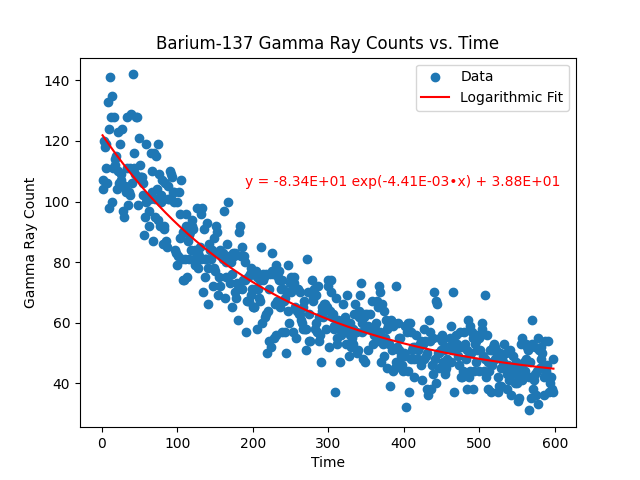
\includegraphics[width=.9\textwidth]{../images/day3_liquidtrial3_plot.png}
\end{figure}

\newpage





\section{Results}

The average half life we measured was $163.1 \pm 8.5$ seconds. This result 
is not totally consistent with the accepted result, but we are within one 
standard deviation of such result. As all of our trials also fell within this
range, we can state that we have observed the half life of Ba-137 correctly.


%=====================================================
%============ Section ================================

\section{Summary and conlcusions}

In this experiment, we observed the average half lifes of samples of Ba-137 to be 
$163.1 \pm 8.5$ seconds. This result is very close to the accepted result.

I would like to thank my lab partner, Sannidhya Desai for his assistance on data
collection and overall assistance. Furthermore, I'd like to thank Dr. Dan Heinzen,
Parth Dave, and Konner Feldman for their assistance throughout the measurement and 
set up processes.

%=====================================================
%============ Bibliography  ==========================
%=====================================================

\begin{thebibliography}{9}

\bibitem{book} R. Feynman, {\it QED}, Ch.7.

\bibitem{article}	
R.Dalitz, Proc. Roy. Soc. (London) {\bf A64}, 667 (1951)

\end{thebibliography}

%=====================================================
%============ End ====================================
%=====================================================

\end{document}

%=====================================================
%============ End ====================================
%=====================================================
